
\subsubsection{Advection vs. Diffusion Sensitivity GDSM Results}

In the parametric sensitivity analysis discussed in section
\ref{sec:AdvVelDiffCoeff}, it was shown that for isotopes of interest, higher
advective velocity and higher diffusivity lead to higher means of the peak
annual dose. However, the relationship between diffusivity and advective
velocity adds depth to the notion of a boundary between diffusive and advective
regimes.

The highly soluble and non-sorbing elements, $I$ and $Cl$ 
were expected to exhibit behavior that is highly sensitive 
to advection in the system in the advective regime but less sensitive to 
advection in the diffusive regime.  

In Figures \ref{fig:VAdvVelI129}, \ref{fig:VAdvVelI129VAdvVel}, 
\ref{fig:VAdvVelCl36}, and \ref{fig:VAdvVelCl36VAdvVel} , $^{129}I$ and 
$^{36}Cl$ are more sensitive to vertical advective velocity for lower vertical 
advective velocities. This demonstrates that for vertical advective velocities 
$6.31\times10^{-6}[m/yr]$ and above, lower reference diffusivities are 
ineffective at attenuating the mean of the peak doses for soluble, non-sorbing 
elements. 

\begin{figure}[htp!]
\begin{minipage}[b]{0.45\linewidth}
\centering
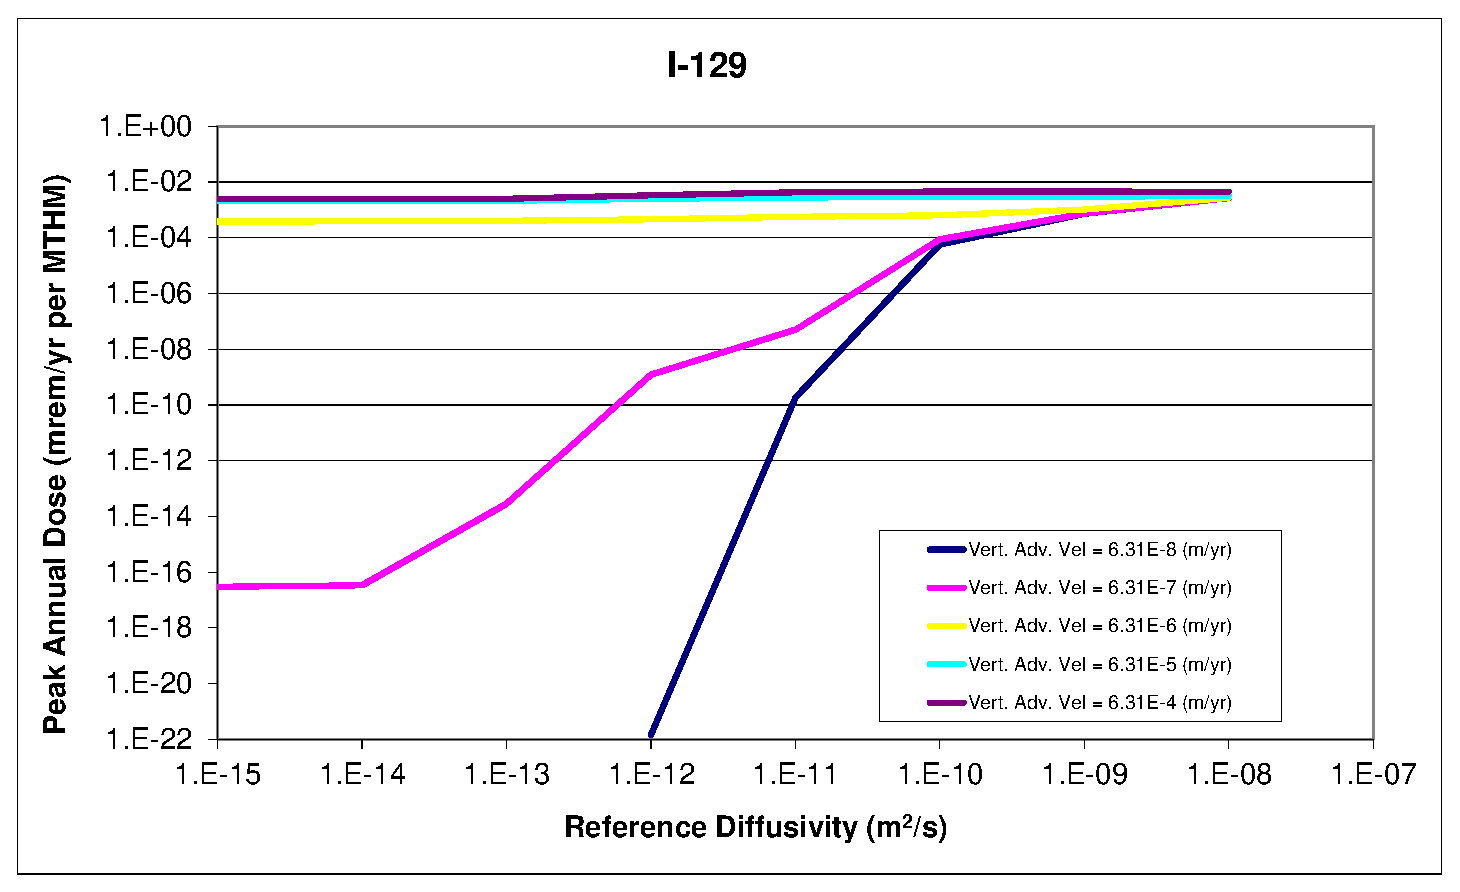
\includegraphics[width=\linewidth]{./chapters/nuclide_sensitivity/clay/AdvVelAndDiffCoeffEBSFail/I-129.eps}
\caption{$^{129}I$ reference diffusivity sensitivity.}
\label{fig:VAdvVelI129}

\end{minipage}
\hspace{0.05\linewidth}
\begin{minipage}[b]{0.45\linewidth}

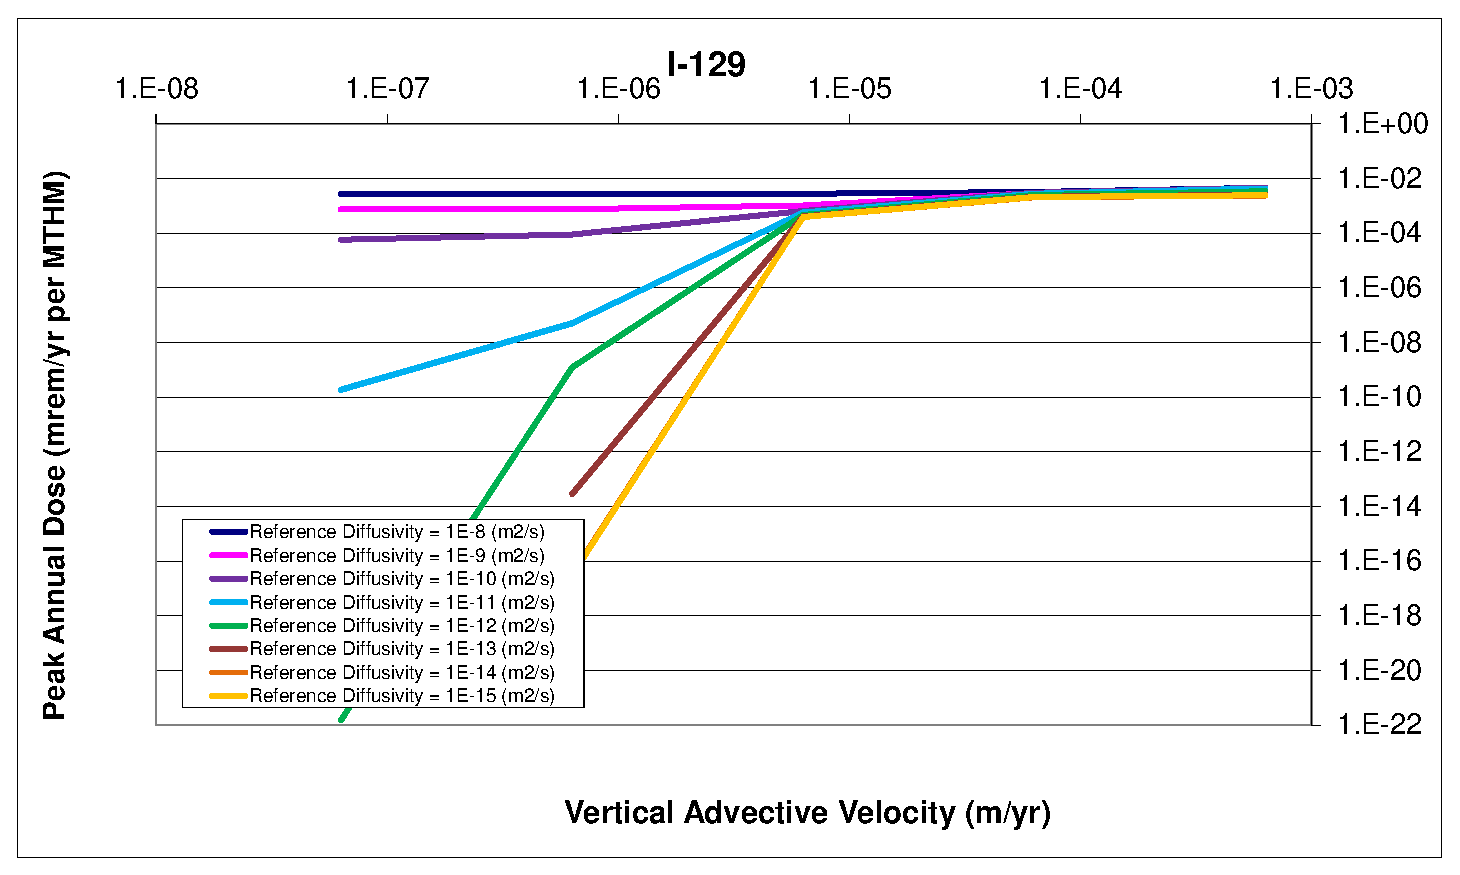
\includegraphics[width=\linewidth]{./chapters/nuclide_sensitivity/clay/AdvVelAndDiffCoeffEBSFail/I-129-VAdvVel.eps}
\caption{$^{129}I$ vertical advective velocity sensitivity.}
\label{fig:VAdvVelI129VAdvVel}

\end{minipage}
\end{figure}

\begin{figure}[htp!]
\begin{minipage}[b]{0.45\linewidth}

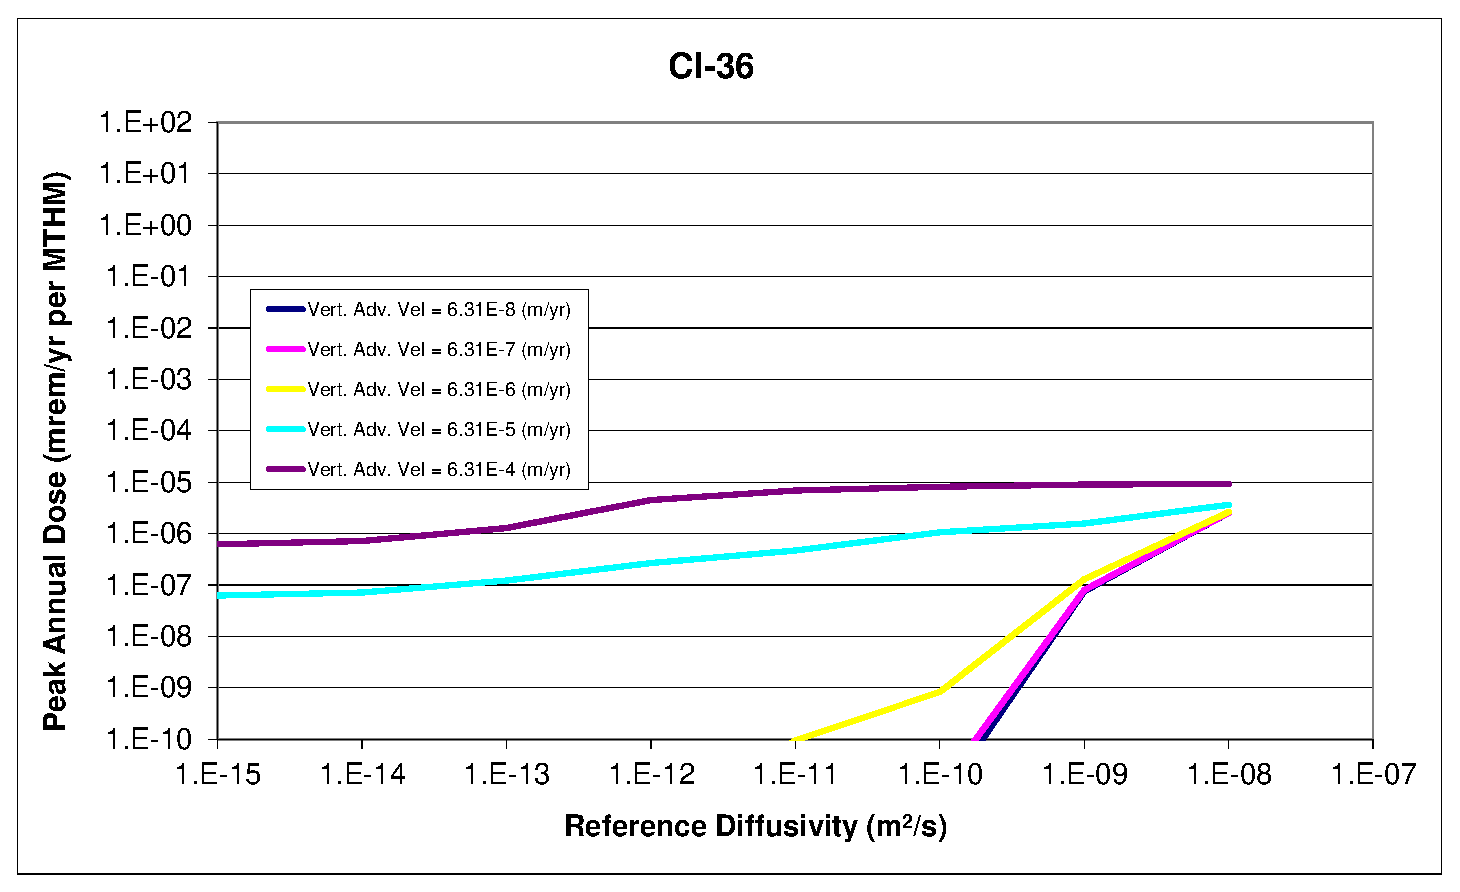
\includegraphics[width=\textwidth]{./chapters/nuclide_sensitivity/clay/AdvVelAndDiffCoeffEBSFail/Cl-36.eps}
\caption{$^{36}Cl$ reference diffusivity sensitivity.}
\label{fig:VAdvVelCl36}

\end{minipage}
\hspace{0.05\linewidth}
\begin{minipage}[b]{0.45\linewidth}

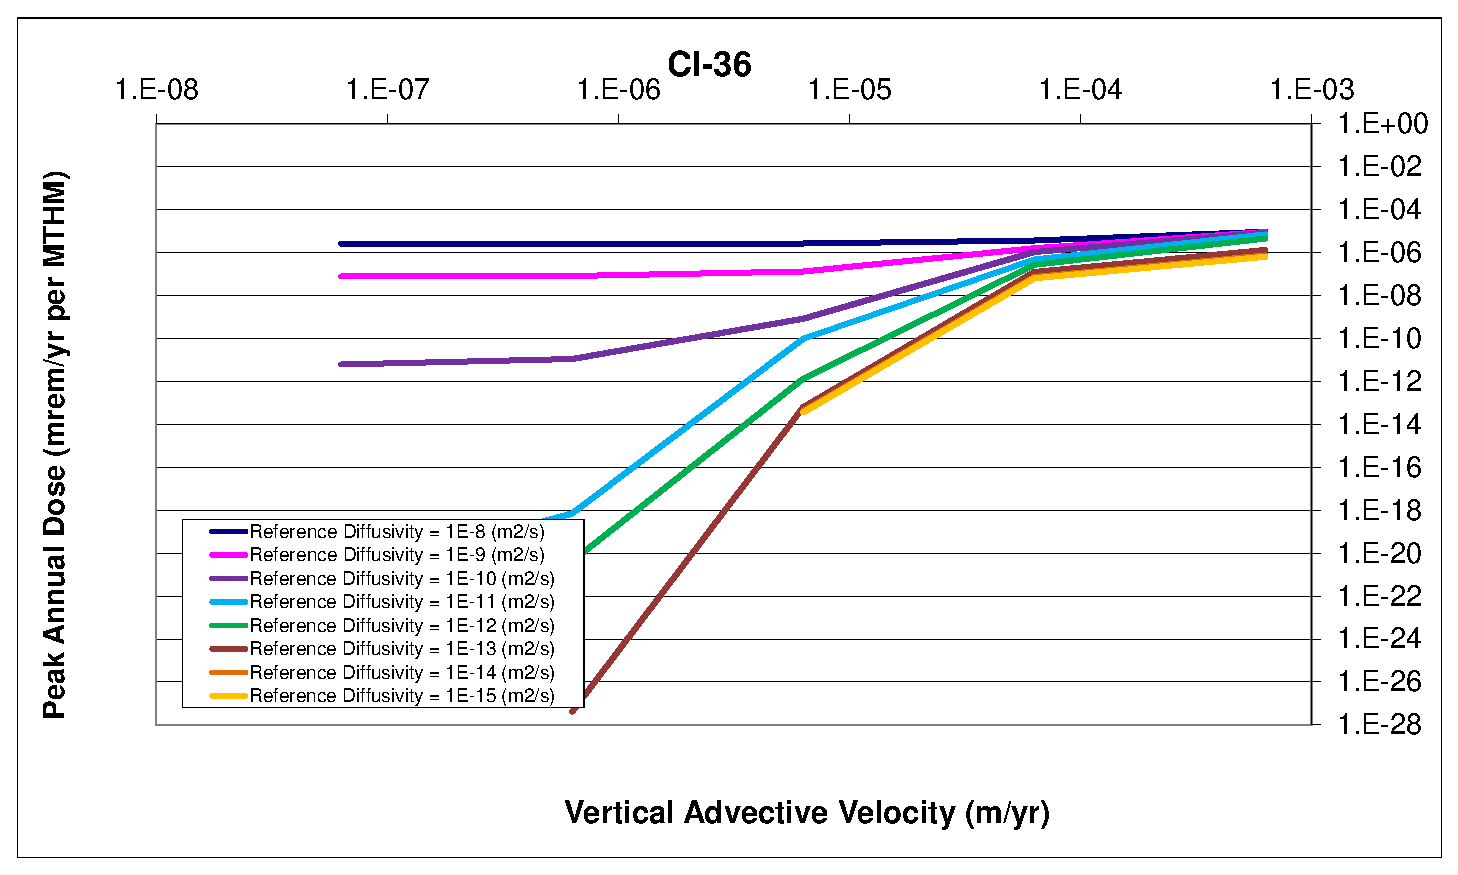
\includegraphics[width=\textwidth]{./chapters/nuclide_sensitivity/clay/AdvVelAndDiffCoeffEBSFail/Cl-36-VAdvVel.eps}
\caption{$^{36}Cl$ vertical advective velocity sensitivity.}
\label{fig:VAdvVelCl36VAdvVel}
\end{minipage}
\end{figure}

The solubility limited and sorbing elements, $Tc$ and $Np$, in Figures 
\ref{fig:VAdvVelTc99}, \ref{fig:VAdvVelTc99VAdvVel}, \ref{fig:VAdvVelNp237}, and 
\ref{fig:VAdvVelNp237VAdvVel} show a very weak influence on peak annual dose 
rate for low reference diffusivities, but show a direct proportionality between 
dose and reference diffusivity above a threshold. For $^{99}Tc$, for example, 
that threshold occurs at $1\times10^{-11}[m^2/s]$. 


Dose contribution from $^{99}Tc$ has a proportional 
relationship with vertical advective velocity above a regime threshold at 
$6.31\times10^{-5}[m/yr]$, above which the system exhibits sensitivity to 
advection. 

%There is an interesting feature in which $^{99}Tc$ 
%exhibits a decrease in peak annual dose for an increase in reference diffusivity 
%for the very high ($6.31\times10^{-4}$) vertcial advective velocity case. %WHY? 

\begin{figure}[htp!]
\begin{minipage}[b]{0.45\linewidth}
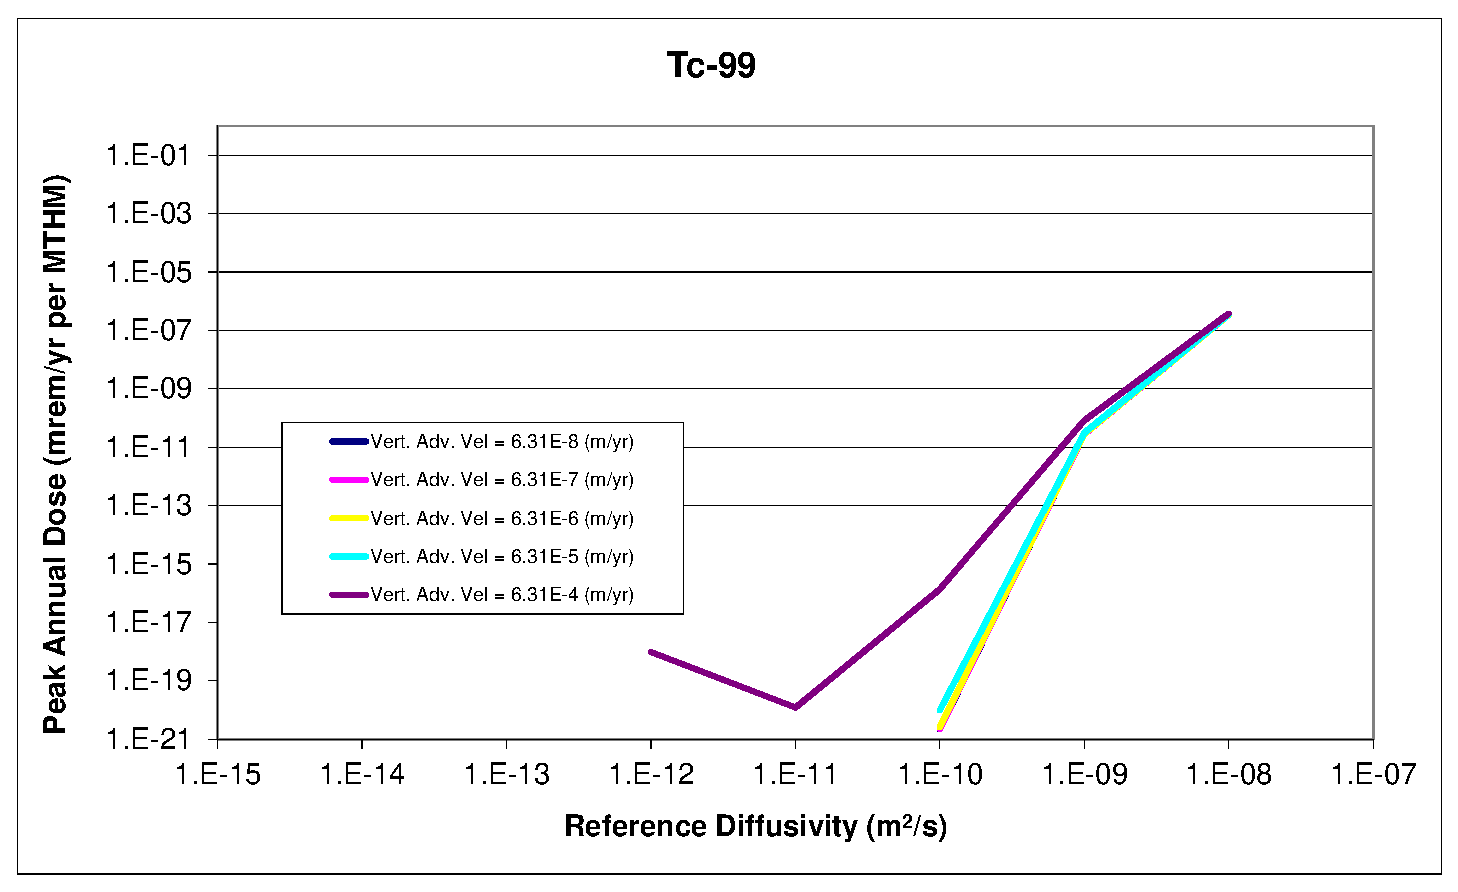
\includegraphics[width=\linewidth]{./chapters/nuclide_sensitivity/clay/AdvVelAndDiffCoeffEBSFail/Tc-99.eps}
\caption{$^{99}Tc$ reference diffusivity sensitivity.}
\label{fig:VAdvVelTc99}

\end{minipage}
\hspace{0.05\linewidth}
\begin{minipage}[b]{0.45\linewidth}

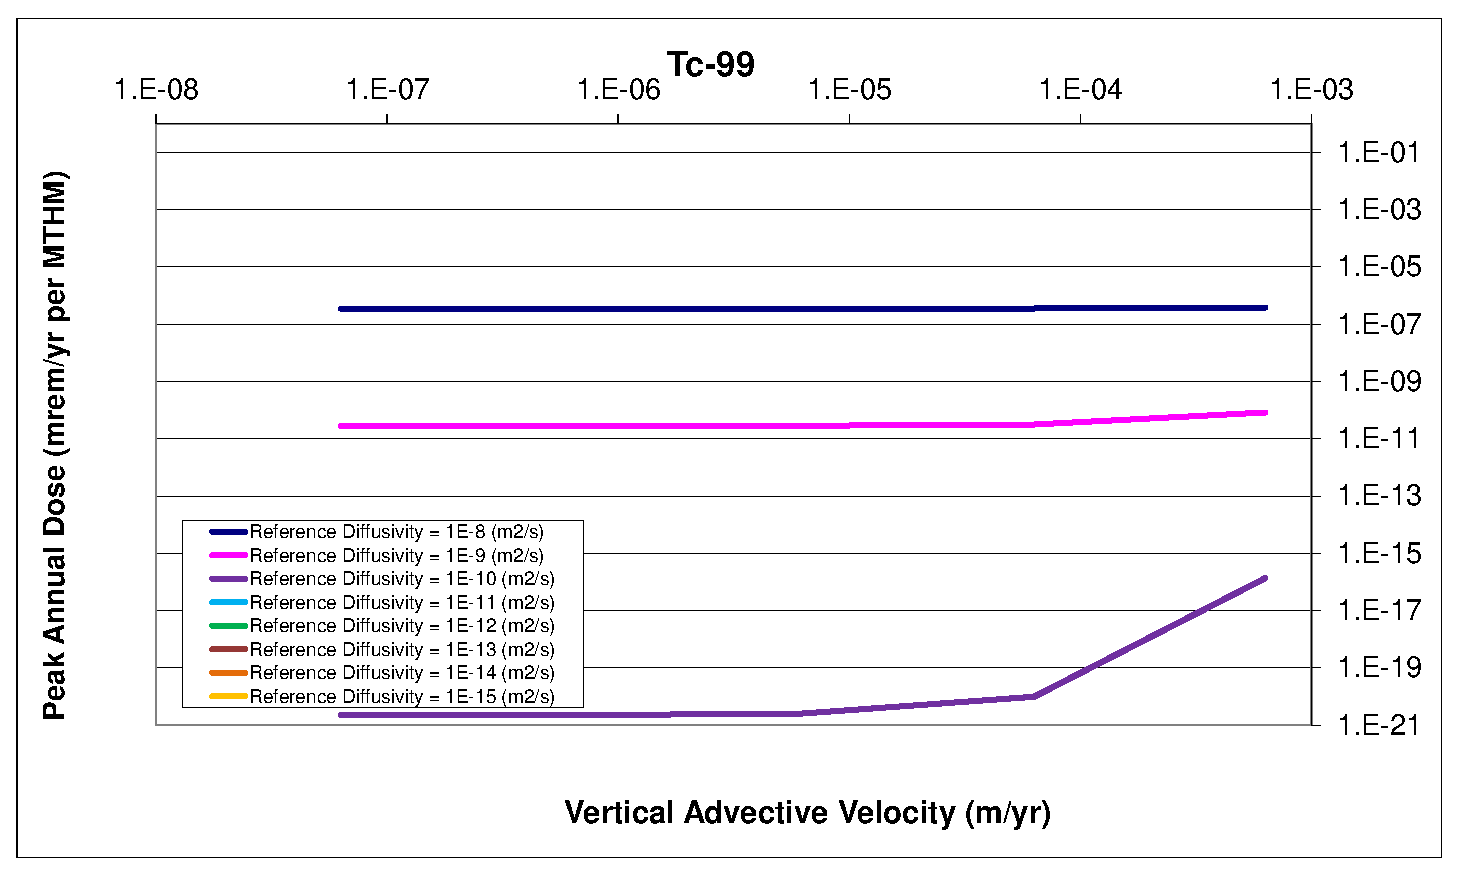
\includegraphics[width=\linewidth]{./chapters/nuclide_sensitivity/clay/AdvVelAndDiffCoeffEBSFail/Tc-99-VAdvVel.eps}
\caption{$^{99}Tc$ vertical advective velocity sensitivity.}
\label{fig:VAdvVelTc99VAdvVel}

\end{minipage}
\end{figure}

\begin{figure}[htp!]
\begin{minipage}[b]{0.45\linewidth}
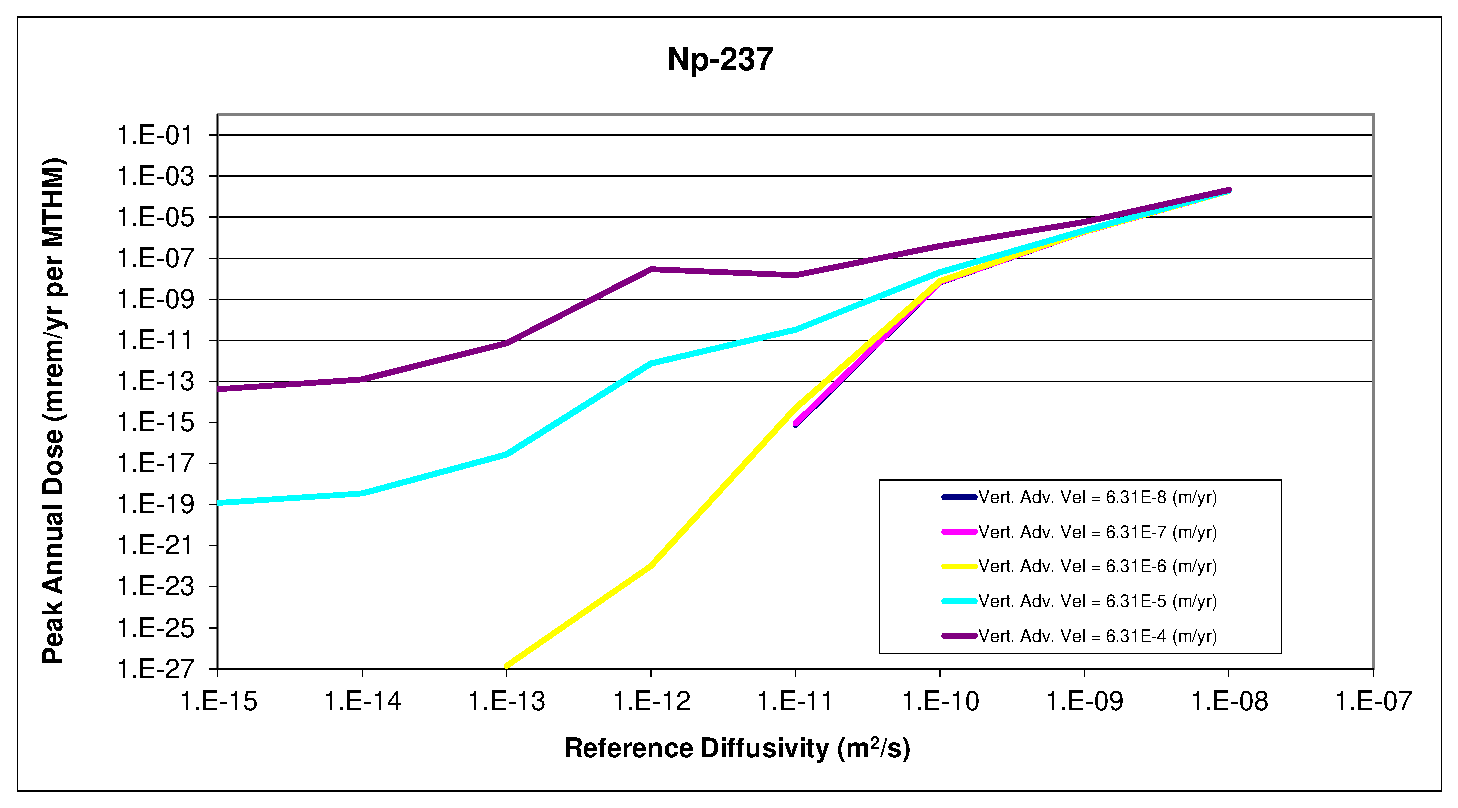
\includegraphics[width=\linewidth]{./chapters/nuclide_sensitivity/clay/AdvVelAndDiffCoeffEBSFail/Np-237.eps}
\caption{$^{237}Np$ reference diffusivity sensitivity.}
\label{fig:VAdvVelNp237}

\end{minipage}
\hspace{0.05\linewidth}
\begin{minipage}[b]{0.45\linewidth}

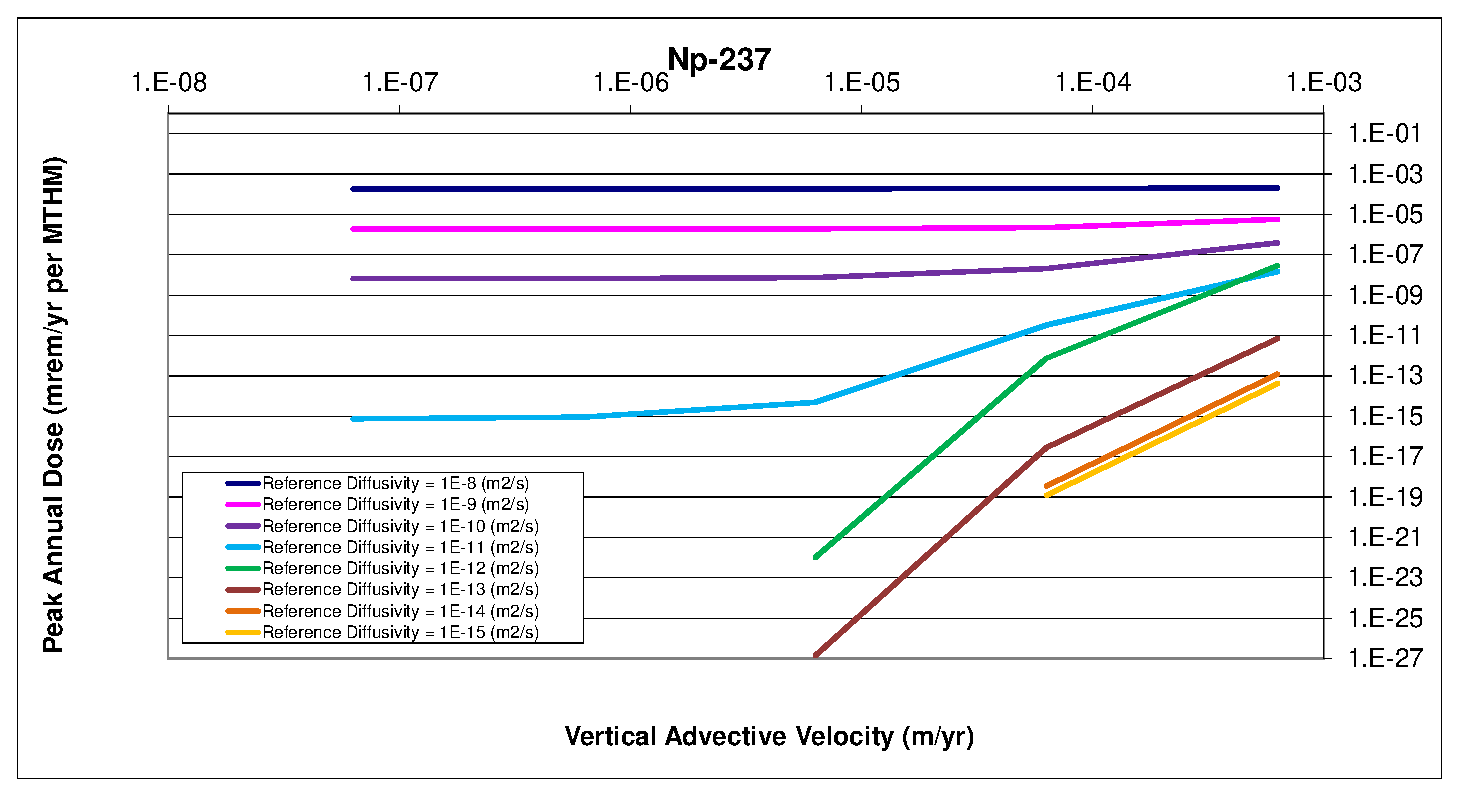
\includegraphics[width=\linewidth]{./chapters/nuclide_sensitivity/clay/AdvVelAndDiffCoeffEBSFail/Np-237-VAdvVel.eps}
\caption{$^{237}Np$ vertical advective velocity sensitivity.}
\label{fig:VAdvVelNp237VAdvVel}
  
\end{minipage}
\end{figure}

The convergence of the effect of the reference diffusivity and vertical 
advective velocity for the cases above shows the effect of dissolved 
concentration (solubility) limits and sorption. $Se$ is non sorbing, but 
solubility limited.  The results from $^{79}Se$ in Figure \ref{fig:VAdvVelSe79} 
and \ref{fig:VAdvVelSe79VAdvVel} show that for low vertical advective velocity, 
the system is diffusion dominated.  However, for high vertical advective 
velocity, the diffusivity remains important even in the advective regime as 
spreading facilitates transport in the presence of solubility limited transport. 

\begin{figure}[htp!]
\begin{minipage}[b]{0.45\linewidth}
\centering
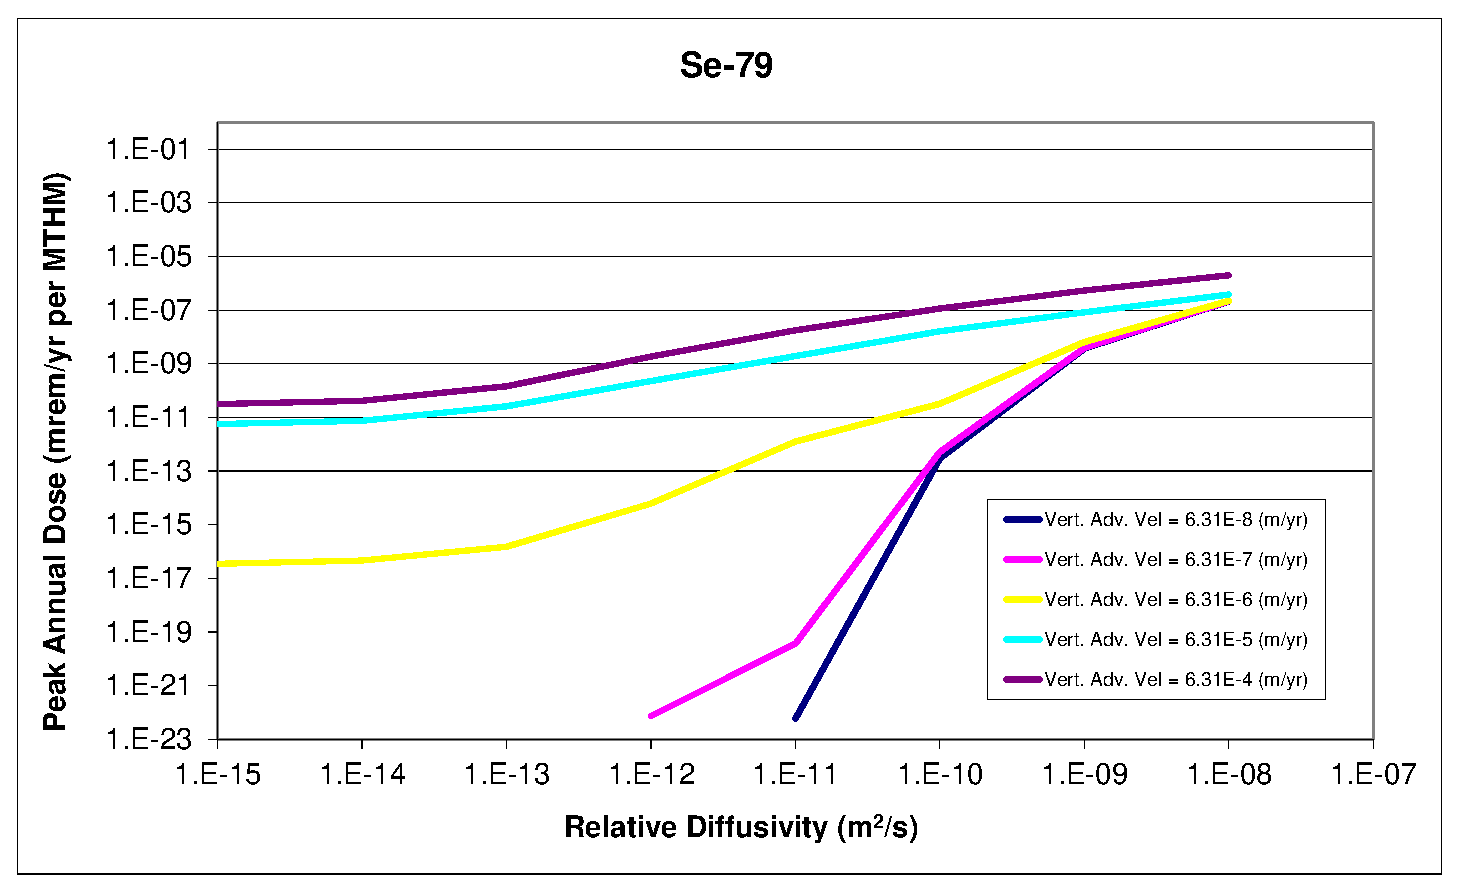
\includegraphics[width=\linewidth]{./chapters/nuclide_sensitivity/clay/AdvVelAndDiffCoeffEBSFail/Se-79.eps}
\caption{$^{79}Se$ reference diffusivity sensitivity.}
\label{fig:VAdvVelSe79}

\end{minipage}
\hspace{0.05\linewidth}
\begin{minipage}[b]{0.45\linewidth}

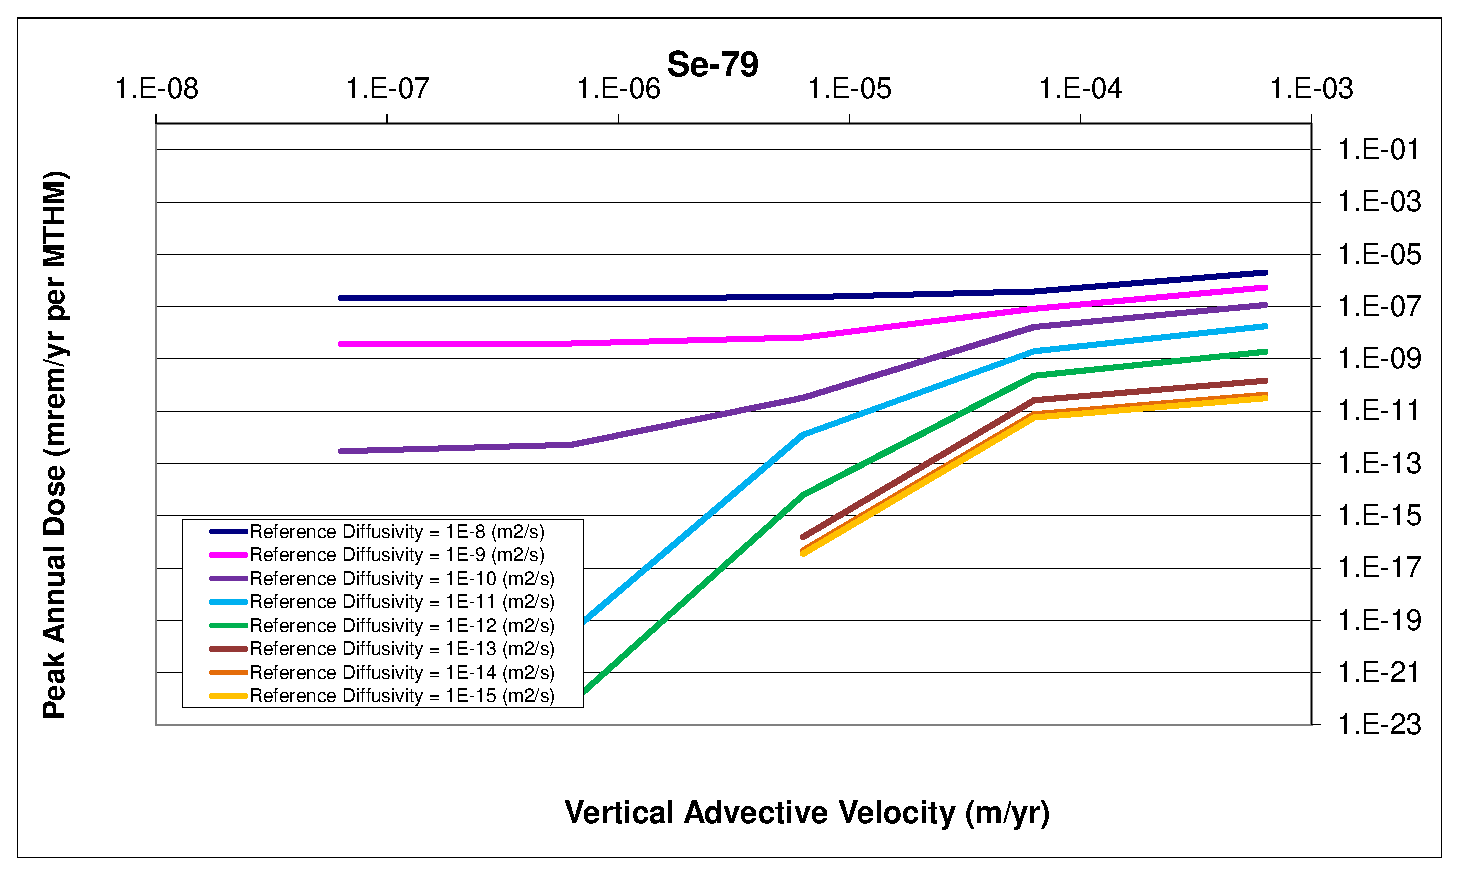
\includegraphics[width=\linewidth]{./chapters/nuclide_sensitivity/clay/AdvVelAndDiffCoeffEBSFail/Se-79-VAdvVel.eps}
\caption{$^{79}Se$ vertical advective velocity sensitivity.}
\label{fig:VAdvVelSe79VAdvVel}

\end{minipage}
\end{figure}
\FloatBarrier
